\chapter{Software Specification}
\label{chap:requirements}
\citet{cadle10} states that there is a standard hierarchical approach in 
structuring requirements. Table \ref{table:requirementsCategories} outlines
the main four categories:

\begin{table}[H]
  \begin{tabular}{|l|l|l|l|}
    \hline
    {\bf General} & {\bf Technical} & {\bf Functional} & {\bf Non-Functional} \\ 
    \hline
    Business constraints & Hardware & Data entry & Performance \\ 
    Business policies & Software & Data maintenance & Security \\ 
    Legal & Interoperability & Procedure & Legal and Access \\ 
    Branding & Internet & Retrieval & Backup and Recovery \\ 
    Cultural & ~ & ~ & Archiving and Retention \\ 
    Language & ~ & ~ & Maintainability \\ 
    ~ & ~ & ~ & Business Continuity \\ 
    ~ & ~ & ~ & Availability \\ 
    ~ & ~ & ~ & Usability \\ 
    ~ & ~ & ~ & Capacity \\
    \hline
  \end{tabular}
  \label{table:requirementsCategories}
\end{table}

Each of the above categories will form the basis of this requirements chapter,
along with any additional user requirements, assumptions and a risk assessment.

% Project Drivers
% Purpose
\newpage
\section{Purpose}

\subsection{Background of the Project}

The purpose of this project is to produce an app that will be compatible with the three main mobile operating systems, iOS, Android and Blackberry OS. The app is to be able to solve given clues from cryptic crosswords which are widely available on publications such as the Burgundian newspaper. There is no current form mobile application in the current market which solves cryptic clues. The produced product is to allow the end user to solve some if not all types of clues which have been discussed in section 2.1.3.

\subsection{Project Goals}

The main goals of the project are:

\begin{enumerate}
  \item Solve a given clue
  \item Produce a mobile interface which shows a stack trace of how the clue was deduced
\end{enumerate}



% Client, customer and stakeholder
\newpage
\section{The Client, the Customer and Other Stakeholders}

\subsection{The Client}

 % Client
	\textbf{Dr Hugh \textsc{Osborne}}\\
	Senior Lecturer\\
	University Of Huddersfield\\
	h.r.osborne@hud.ac.uk

\subsection{The Customer}

The intended customer of the product are users of smartphone and tablets whom are looking to solve all those unsolvable Cryptic Crosswords. The applications will be deployed on the app market for the three listed mobile operating systems which means that the app will be available to anyone who has a compatible device with the required software. The physical deployment of the application is out of the project scope so a price for the deployment will not be discussed.

\subsection{Other Stakeholders}

For the purpose of the project the other stakeholders are as follows:

 % Supervisor
      \emph{Project Supervisor}\\
      \textbf{Dr. Gary \textsc{Allen}} \\
      Senior Lecturer \\
      University Of Huddersfield \\
      g.allen@hud.ac.uk 

  % Examiner
      \emph{Project Examiner:} \\ 
      \textbf{Sotirios \textsc{Batsakis}}\\
      University Of Huddersfield\\
      s.batsakis-STA@unimail.hud.ac.uk

  % Moderator
      \emph{Internal Moderator}\\
      \textbf{Collin \textsc{Venters}} \\
      Senior Lecturer \\
      University Of Huddersfield \\
      c.venters@hud.ac.uk



% Project Constraints
% Mandated Constraints
\newpage
\newpage
\section{Mandated Constraints}

The following section describes the constraints that effect the design of the
product. The product that is to be developed cannot be successful unless these
constraints have been accomplished.

%Solution Constraints
\subsection{Solution Constraints}

\noindent\llap{\textbf{[R1/1]}}The product shall be built for the following platforms:\\
\begin{enumerate}
		\item Blackberry
		\item iOS 
		\item Android
\end{enumerate}

\textbf{Rationale:}  The product it to be able to be used on the go.\\
\textbf{Volatility:} High


\noindent\llap{\textbf{[R2/1]}}The product shall require an Internet connection. \\

\textbf{Rationale:}  The product cannot work without an Internet connection.\\
\textbf{Volatility:} High

%Implementation Environment of the System
\subsection{Implementation Environment of the System}

\noindent\llap{\textbf{[R3/1]}}The product shall run on the following operating systems:\\

\begin{enumerate}
		\item Blackberry 10.2
		\item iOS 7
		\item Android 4.2 Jellybean
\end{enumerate}

\textbf{Rationale:}  The product is new therefore run on the latest software\\
\textbf{Volatility:} High

%Partner or Collaborative Applications
\subsection{Partner or Collaborative Applications}

\noindent\llap{\textbf{[R4/1]}}The product shall allow the user to login with their facebook account.

\textbf{Rationale:}  The product will allow a user to login in order to keep a search history, instead of creating a new authentication the user should be able to login using third part applications\\
\textbf{Volatility:} Low

%Off-the-Shelf Software
\subsection{Off-the-Shelf Software}

\noindent\llap{\textbf{[R5/1]}}The product shall make use of the Apache OpenNLP Library.

\textbf{Rationale:}  In order for the product to recognize the clues the best possible technique is to use Natural Language processing tools.\\
\textbf{Volatility:} Medium

%Schedule Constraints
\subsection{Schedule Constraints}

\noindent\llap{\textbf{[R6/1]}}The product shall be completed on or before the 18th April 2014.

\textbf{Rationale:}  The final deadline for all deliverables are 18/04/2014. \\
\textbf{Volatility:} High

%Budget Constraints
\subsection{Budget Constraints}

\noindent\llap{\textbf{[R7/1]}}The product shall be developed using all freely available tools and the only constraint of budget shall be the time the project resources put into to the product.

\textbf{Rationale:}  As the resources of the project are students, the product needs to be developed using the least amount of money as possible. The necessary steps should be taken to ensure that no costs are accumulated while developing the product \\
\textbf{Volatility:} Medium



% Naming_Conventions And Terminology 
\newpage
\section{Naming Conventions and Terminology}

The following section contains a glossary with the meanings of all names, acronyms, and abbreviations used by the stakeholders.

\newpage
\subsection{Definitions of All Terms}

\begin{table}
    \begin{tabular}{|l|l|}
    \hline
    Term/Acronym  & Definition                                                \\ \hline
    The Guardian  &  A newspaper with a website featuring cryptic  crosswords \\ \hline
    Blackberry    & A mobile phone platform by Blackberry                     \\ \hline
    iOS           & A mobile phone platform by Apple                          \\ \hline
    Android       & A mobile phone platform by  Google                        \\ \hline
    NLP           & Natural Language Processing                               \\ \hline
    SRS           & Software Requirements Specification                       \\ \hline
    App           & Short for application                                     \\ \hline
    ~             & ~                                                         \\ \hline
    ~             & ~                                                         \\ \hline
    ~             & ~                                                         \\ \hline
    ~             & ~                                                         \\ \hline
    ~             & ~                                                         \\ \hline
    ~             & ~                                                         \\ \hline
    ~             & ~                                                         \\ \hline
    \end{tabular}
\end{table}



% Relevant_Facts_And_Assumptions
\newpage
\section{Relevant Facts and Assumptions}

\subsection{Facts}

\noindent\llap{\textbf{[I1/1]}}Answers to Cryptic Crosswords are usually published the following day

\noindent\llap{\textbf{[I2/1]}}The same clues does not always have the same answers

\noindent\llap{\textbf{[I3/1]}}Existing applications don't offer real time solvers

\noindent\llap{\textbf{[I4/1]}}Electronic solvers not available

\subsection{Assumptions}

\begin{enumerate}
\item Equipment needed to test the application on different platforms will be
available.
\item A server to host the web service will be available.
\item The Guardian has given permission to use their cryptic crossword data to use for
our test data.
\item Four team members working on the project throughout the year at approximately
25\% of their academic study time
\item Project scope will remain the same throughout the project
\end{enumerate}


% Functional Requirements
% The Scope of the Work
\newpage
\newpage
\section{The Scope of the Work}

The following sections define the roles and processes of the team developing the Cryptic Crossword Solver. 

\subsection{Organization Structure}

The project team is based largely upon democratic discussions and decisions, however to ensure that team deadlocks do not occur a project leader has been chosen. Figure ~\ref{fig:org_hierachy} reflects the hierarchy of the team.


\begin{figure}[here]
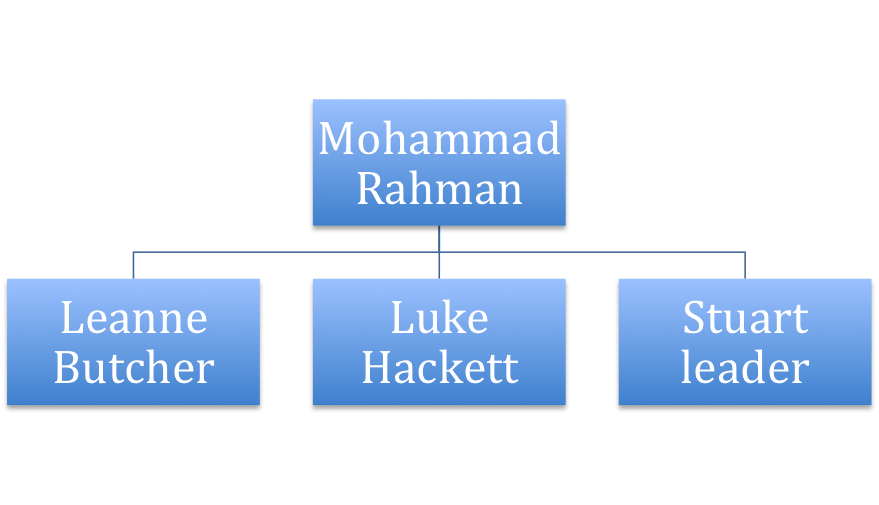
\includegraphics[width=0.9\textwidth]{requirements/functional_requirements/org_hierachy.png}
\caption{Hierarchical Structure of the team}
\label{fig:org_hierachy}
\end{figure}


\subsection{Methodology}

It has been decided that the team will follow an Agile software development model. This will allow the team to split the larger task down into smaller, more manageable ‘chunks’, that allows for a good quality analysis, evaluation, development and planning (on to the next ‘chunk’). An iterative approach is best suited for this project due to the nature of changes and updates the product will require in future builds.

This method of development also allows for a more feature-driven approach to the project. Ultimately this allows for more important features and aspects of the project to be completed first. 

Include diagram <here>


\subsection{Meetings}

A weekly meeting will take place between all project members to discuss all aspects of the project. This includes (but is not limited to) project issues, software development issues, research findings, possible improvements and code reviews.



% Business Data Model & Data Dictionary
\newpage
\section{Business Data Model \& Data Dictionary}

% The Scope of the Product
\newpage
\section{The Scope of the Product}

\subsection{Use case Diagrams}

% Functional Requirements
\newpage
\section{Functional Requirements}


\subsection{Data entry}

\subsection{Data maintenance}

\subsection{Procedure}

\subsection{Retrieval}



%Non-functional Requirements
%Look and Feel Requirements
\newpage
\section{Look and Feel Requirements}

%Usability and Humanity Requirements
\newpage
\section{Usability and Humanity Requirements}

%Performance Requirements
\newpage
\section{Performance Requirements}

% Operational and Environmental Requirements
\newpage
\section{Operational and Environmental Requirements}


%Maintainability and Support Requirements
\newpage
\section{Maintainability and Support Requirements}

%Security Requirements
\newpage
\section{Security Requirements}

%Cultural Requirements
\newpage
\section{Cultural Requirements}

%Legal Requirements
\newpage
\section{Legal Requirements}

%Project Issues
%Open Issues
\newpage
\section{Open Issues}
%Off-the-Shelf Solutions

\newpage
\input{requirements/project_issues/Off_the_shelf_solutions}

%New Problems
\newpage
\section{New Problems}

%Tasks
\newpage
\section{Tasks}

%Migration to the New Product
\newpage
\section{Migration to the New Product}

%Risks
\newpage
\section{Risk Assessment}

% Introduction.
An investigation into the potential risks that may present themselves during the course of this project is of paramount importance if their impact is going to be minimised, should they become a reality.

% Included here a risk impact table
\subsection{Risk Identification}

% PI Scores and risk classification graph
\subsection{Risk Classification}

\subsection{Risk Prevention}

\subsection{Risk Mitigation}

%Costs
\newpage
\section{Costs}

%User Documentation and Training
\newpage
\section{User Documentation and Training}

%Waiting Room
\newpage
\section{Waiting Room}

%Ideas for Solutions
\newpage
\section{Ideas for Solutions}


